\chapter{Parallel Computing}
\label{ch:parallel_computing}
\dictum[Immanuel Kant]{%
	Sapere aude! Habe Mut, dich deines eigenen Verstandes zu bedienen! }%
\vskip 1em
%\section{Introduction}
\lettrine[lines=3,lhang=0.33,lraise=0,loversize=0.15]{O}{ver} the last two decades lot has changed regarding the way modern scientific applications are designed, written and executed especially in the field of data-analytics, modelling and simulation and visualization mainly because the size of the problems that scientist try to tackle nowadays are much bigger and because of the amount of available raw data that can be analyzed. 
Traditionally performance improvements in computer architecture have come from cramming ever more functional units onto silicon, increasing clock speeds and transistors number. Moore's law states that the number of transistors that can be placed inexpensively on an integrated circuit will double approximately every two years (See Figure \ref{fig:moore}). Coupled with increasing clock speeds CPU performance has until recently scaled likewise. But it is important to acknowledge that this trend cannot be sustained indefinitely or forever. Increased clock speed and transistor number require more power and consequently generate more heat. Although the trend for transistor densities has continued to steadily increase, clock speeds began slowing circa 2003 at 3 GHz. If we apply Moore’s law type thinking to clock-speed performance, we should be able to buy at least 10 GHz CPUs. However, the fastest CPU available at the time of writing is $\approx 4.0 GHz$.
\begin{figure}
\centering
%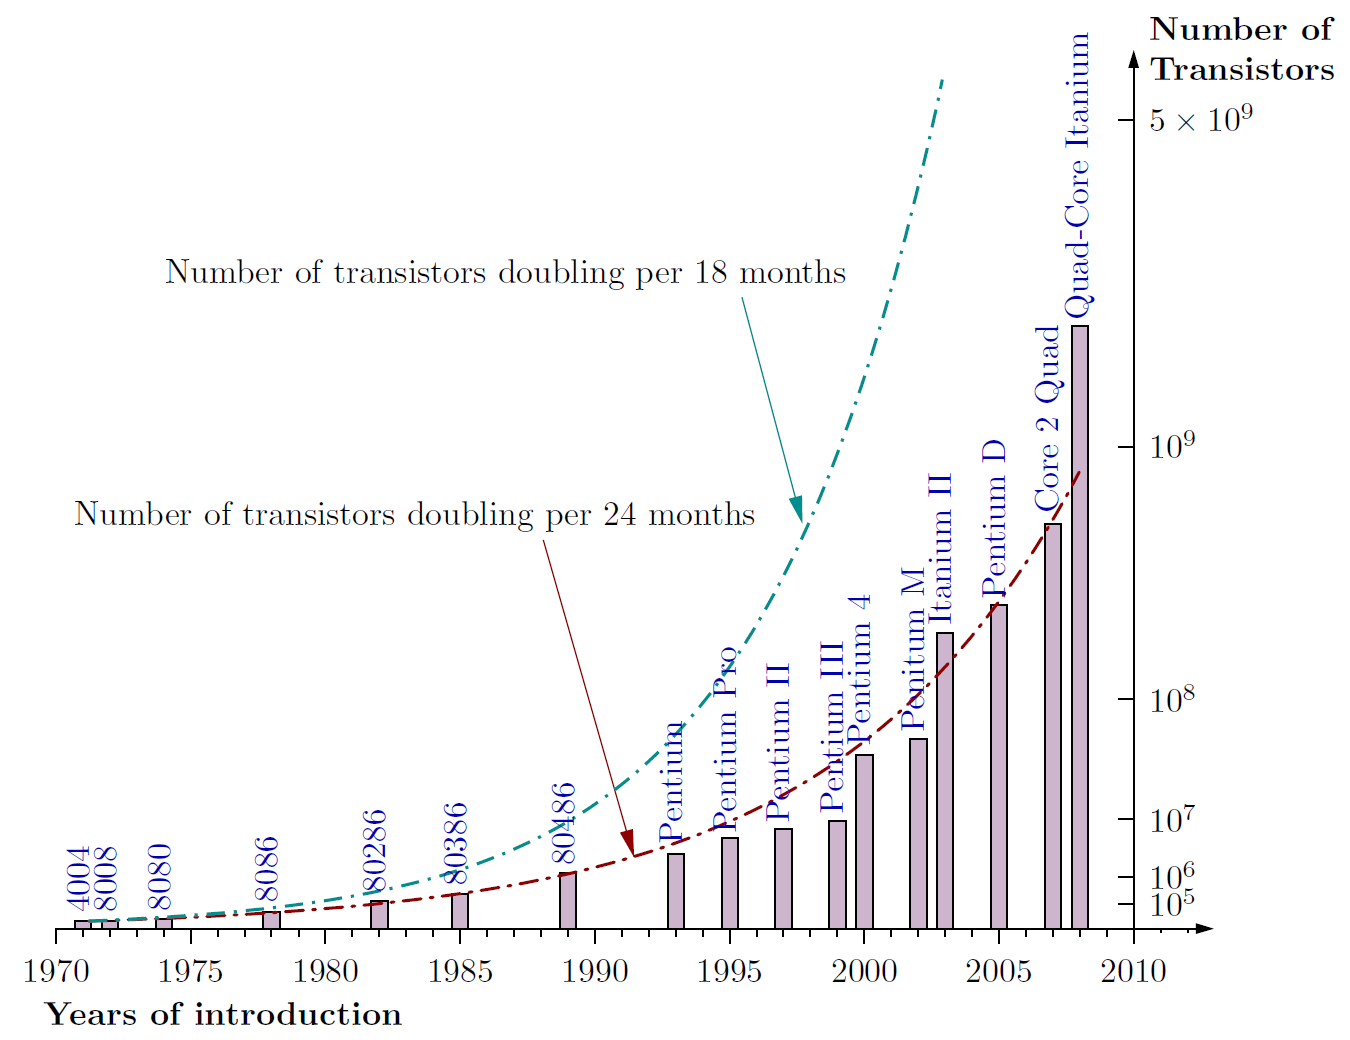
\includegraphics[totalheight=0.5\textheight]{./images/parallel_programming/moore_law_large}
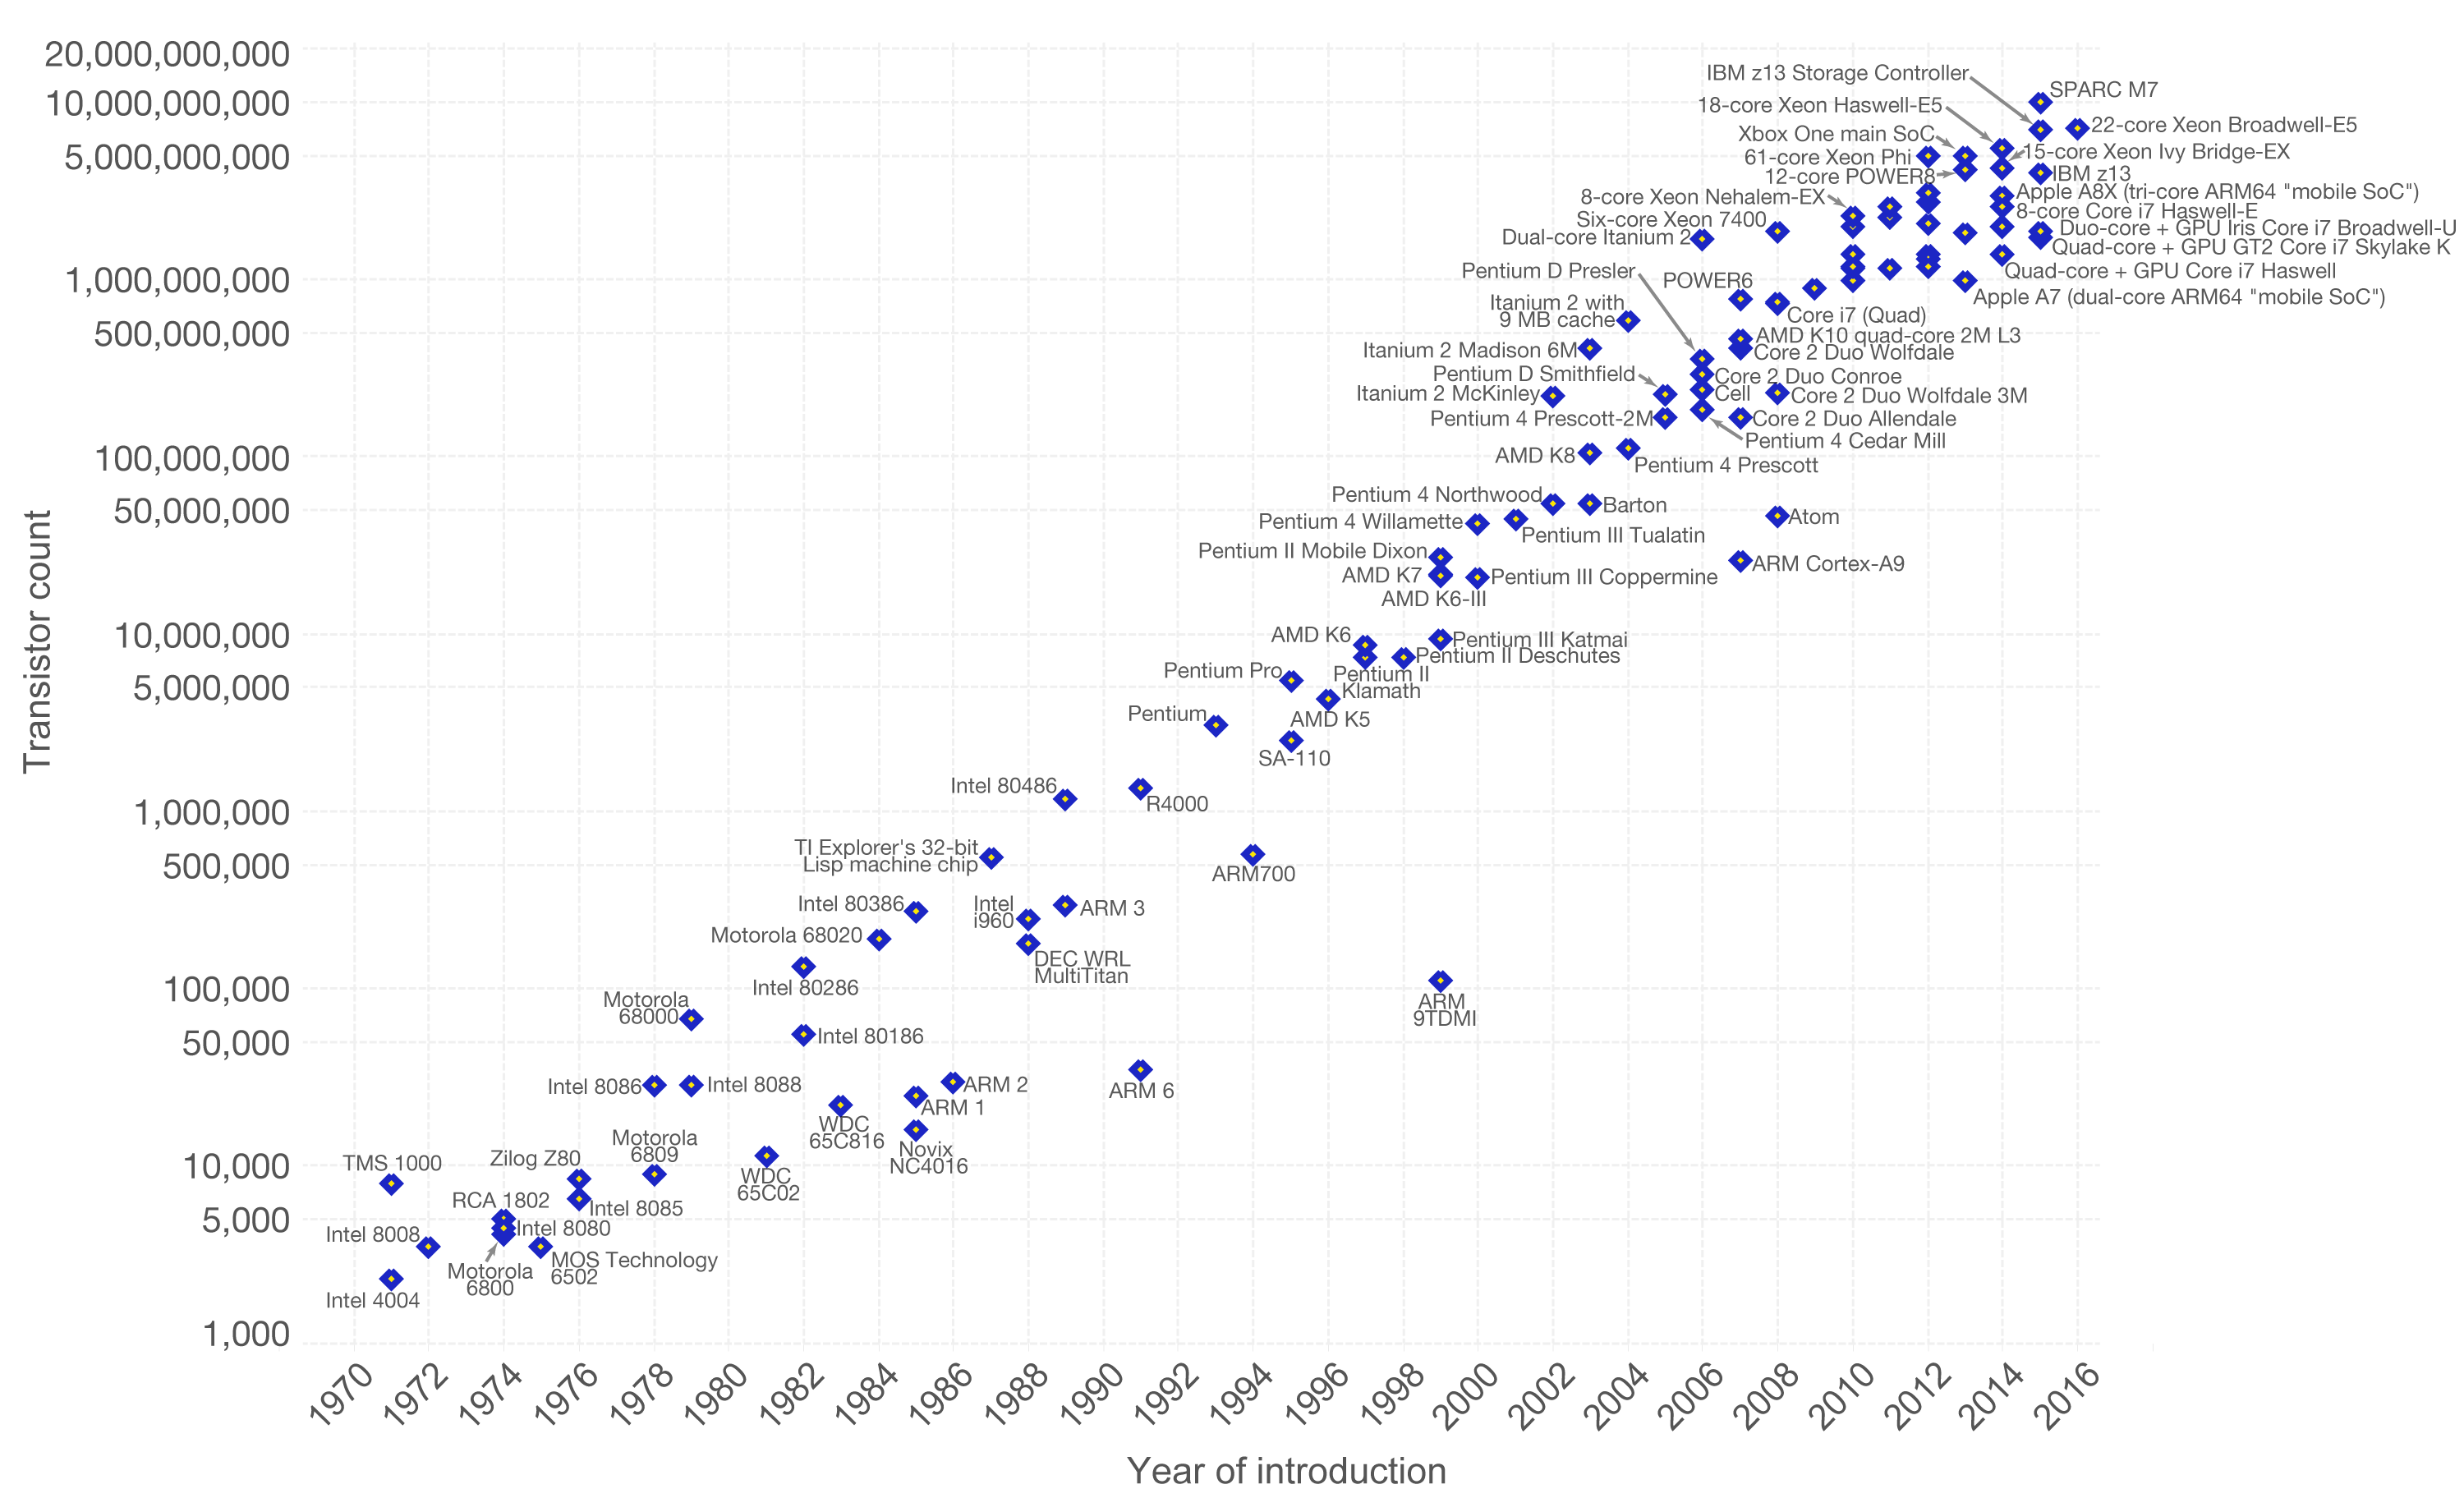
\includegraphics[width=1.0\textwidth]{./images/parallel_programming/moore_law2}
\caption{Moore's Law regarding CPU transistors number
history.}\label{mooreLaw}
\end{figure}
At same point the performance gaining fails to increase proportionally with the added effort in terms of transistors number or clock speed because efficient heat dissipation and increasing transistor resolution on the wafer, which is not far from from its physical limit (the atom scale),  becomes more important and challenging.
The heat emitted from the modern processor, measured in power density rivals the heat of a nuclear reactor core (see Figures \ref{fig:tempCPU} and \ref{fig:tempCPU_thermal})!
\begin{figure}
	\centering
	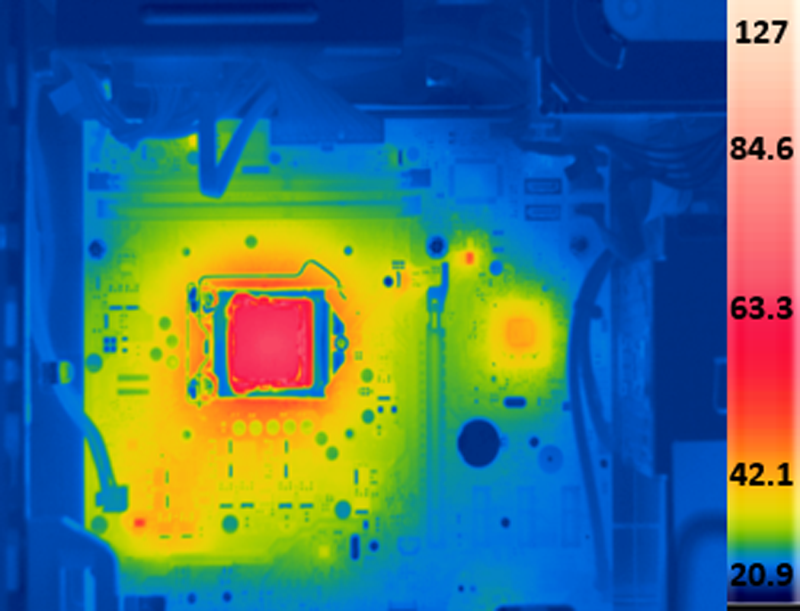
\includegraphics[width=1.0\textwidth]{./images/parallel_programming/heat_cpu}
	\caption{Thermal camera image of a modern CPU showing that heat is concentrated in a small part of the wafer.}\label{fig:tempCPU_thermal}
\end{figure}
But the power demand did not stop in these year, and is not going to stop in the near future, here the necessity of relying heavily on parallel architectures, so today the dominating trend in commodity CPU architectures is multiple processing cores mounted on a single die operating at reduced clock speeds and sharing resources and memory. Today is normal to use multicore (2,4,8,12, up to 40) CPUs on a desktop PC at home at the point that is very uncommon to be able to buy a single core device.
Even smartphones are proper multicore machines; for instance, the popular mobile CPU \textit{Snapdragon 835} manufactured by Qualcomm is a $8 \times$ cores each of them with a clock speed up to $2.45$ GHz.
\begin{figure}
\centering
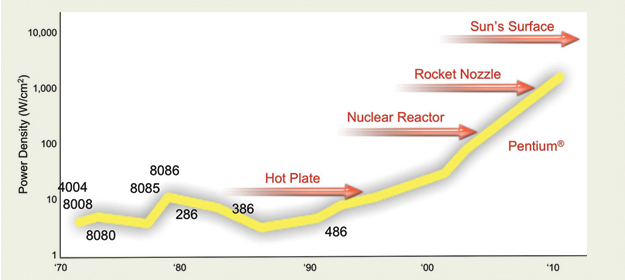
\includegraphics[width=1.0\textwidth]{./images/parallel_programming/temperatureCPU}
\caption{Temperature density CPUs}\label{fig:tempCPU}
\end{figure}



Lot of effort has put during these years in order to try to mitigate and overcome the limits regarding the sequential computer architecture which may derive from its three main components:
\begin{enumerate}

\item  Processor

\item Memory

\item  Communication system (datapaths, usually buses)
\end{enumerate}
All three components present bottlenecks that limit the overall computing performance capability of a system. Caches, low-latency high bandwidth and small capacity memories, for example can hide latency of DRAM chips storing the fetched data and serving subsequent requests of the same memory location\footnote{The fraction of the data satisfied by the cache is called \textit{\textbf{hit rate}}.}. But one of the most important innovation that addresses these bottlenecks is multiplicity (in processor, memories and datapaths) that allows to extend the class of tractable problems with larger instances and more cases that can be handled. This multiplicity has been organized in several manners during the years giving birth to a variety of architectures.

\section{Architectures}
Lots of definitions and classifications have been proposed in years, mostly based on the adopted hardware configuration or logical approach in handling and implementing the parallelism, in order to categorize parallel systems.Among all, Flynn's taxonomy seems to be a well known and accepted one and is here introduced briefly.
\subsection{Classical classification - Flynn's taxonomy}
\label{sec:flynn_tax}
The classification is based on the notion of  \textit{stream of information}.
Two types of information flow into the processor: instructions and data.
Conceptually they can be separated into two independent streams. A coarse
classification can be made taking in account only the number of instructions and
 data streams that a parallel machine can manage (see figure \ref{fig:parallelClassification1}).
That's how Flynn's taxonomy\cite{Flynn1972} classifies machines: according to
whether they have one or more streams of each type.
\begin{figure}
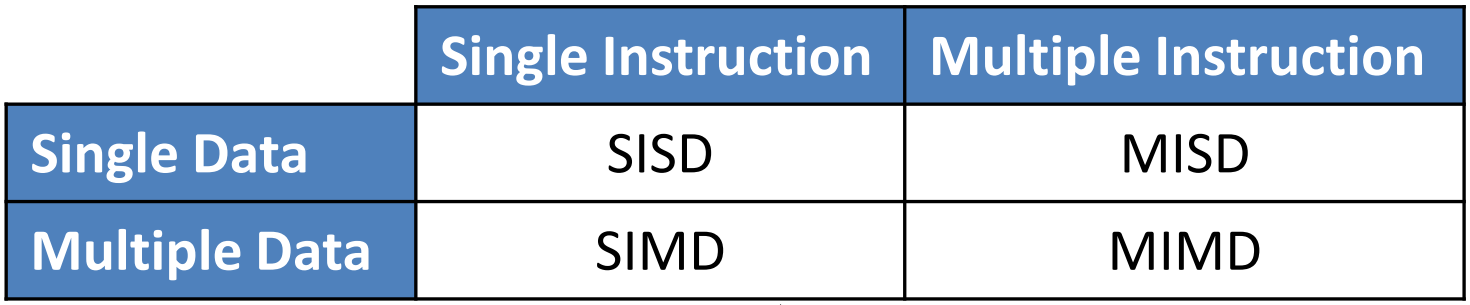
\includegraphics[width=1.0\textwidth]{./images/parallel_programming/parallelClassification}
\caption[Flynn's Parallel architecture taxonomy]{Flynn's Parallel architecture taxonomy.}
\label{fig:parallelClassification1}
\end{figure}
\begin{description}
\item[SISD:] \textit{\textbf{Single}} instruction \textit{\textbf{Single}}
data.\hfill\\
No parallelism in either instruction or data streams. Each arithmetic
instruction initiates an operation on a data item taken from a single stream of data elements (e.g. mainframes). A single control unit fetches a single instruction from the memory.
\item[SIMD:] \textit{\textbf{Single}} instruction
\textit{\textbf{Multiple}} data. \hfill \\ Data parallelism. The same
instruction is executed on a batch of different data. The control unit is
responsible for fetching and interpreting instructions. When it encounters an
arithmetic or other data processing instruction, it broadcasts the instruction
to all processing elements (PE), which then all perform the same operation. For
example, the instruction might be \textit{add R3,R0.}. Each PE would add the
contents of its own internal register R3 to its own R0. (e.g. stream
processors\footnote{Vector processing is performed on an SIMD machine by distributing
elements of vectors across all data memories.}.) SSE and AVX extensions to the $x86$ processors family is an example of such parallelism. One single instruction can operate on up to $512$ byte of data (see Figure \ref{fig:SSEvectorization}). SIMD exploits data and spatial prallelism in a synchronous manner.

\begin{figure}
	\centering
	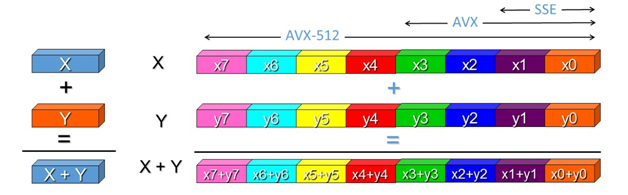
\includegraphics[width=1.0\textwidth]{./images/parallel_programming/vectorization_example}
	\caption{Example of vectorization with Intel SSE and extension.}
	\label{fig:SSEvectorization}
\end{figure}

\item[MISD:] \textit{\textbf{Multiple}} instruction \textit{\textbf{Single}} data. \hfill \\ 
Multiple instruction operating on the same data stream  (See Figure \ref{fig:MISD}). It is a class of system very unusual, mostly for fault-tolerance reasons. No machines in this category have been commercially successful or had any impact on computational science. 
An type of of computer  that fits the MISD description is the so called \textit{systolic array} which consists of a network of pipelined primitive computing nodes or processors. 
\begin{figure}
	\centering
	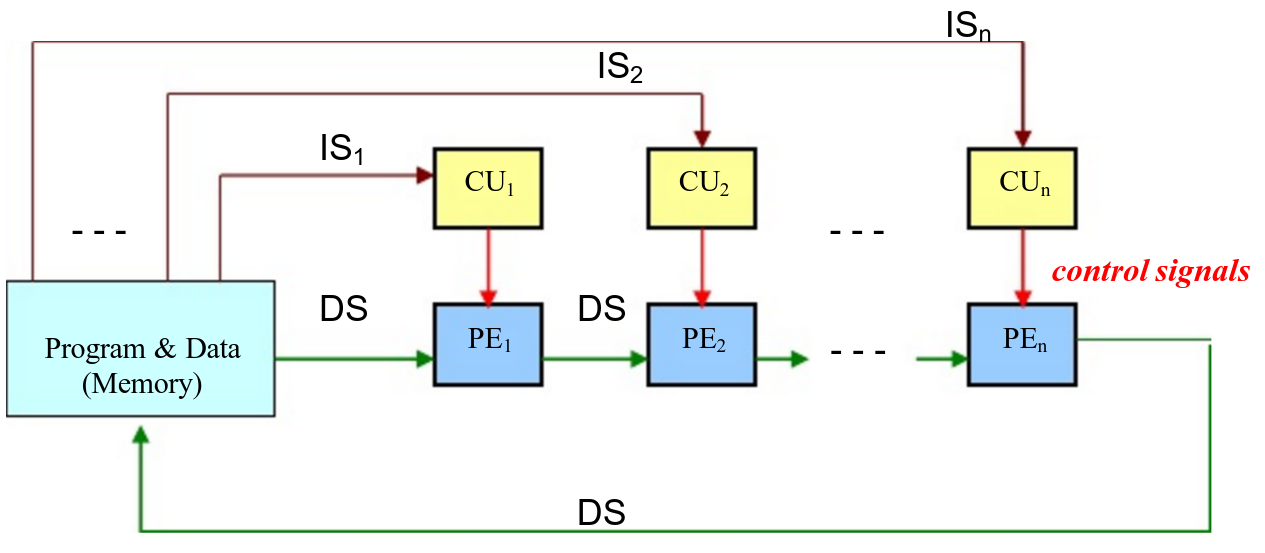
\includegraphics[width=1.0\textwidth]{./images/parallel_programming/MISD}
	\caption{MISD machine schematization. Each processor $CU_i$ has its own instruction flow and all operates on the same data.}
	\label{fig:MISD}
\end{figure}
 
\item[MIMD:] \textit{\textbf{Multiple}} instruction

\textit{\textbf{Multiple}} data. \hfill \\ Multiple instruction operating
independently on multiple data streams (e.g. most modern computers). A MIMD machine is an example of a true multiprocessor and are often employed to ro perform the so called \textit{Single Program Multiple Data} computation where each independent processor executes the same program.
MIMD architecture can be further divided by by their memory layout and organization:
\begin{description}
	\item [Shared Memory (modern CPUs)] where each processors shares the same memory address space and are interconnected by a shared buses. 	Shared memory architecture ar usually shipped as \textit{Symmetric Multi Processors} (SMP) since each of them is usually identical in computational and access to resources capabilities, and the OS kernel can run on any of them in contrast to \textit{Asymettric Multiprocessor} where there is a master-slave relationship  among the group of processors. According to whether subsets of processors have a dedicated and private memory module we can categorize SM architectures in:	
	\begin{itemize}
		\item UMA (Uniform Memory Access) : Identical processors with equal
		access time to memory (see figure \ref{fig:UMA_NUMA}),
		sometimes called CC-UMA acronym for Cache Coherent UMA, because the
		hardware ensures that all the processor can see a memory modification
		performed by one of them.
		\item NUMA (Non Uniform Memory Access): Usually different groups
		of processors (SMP, Symmetric multiprocessors\footnote{Group of processors connected via buses. Usually they consist of not more than 32 processors.}) are connected, and processors belonging to different SMP can access memoryspaces of each others. As NUMA if is present a cache coherence mechanism this architecture is called CC-NUMA.
		 \begin{figure}
			\caption{Shared memory architectures.}
			\label{class12}
			\centering
			\begin{subfigure}[b]{0.5\textwidth}
				\centering
				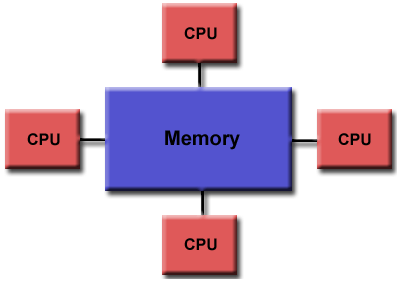
\includegraphics[width=0.92\textwidth]{./images/parallel_programming/shared_mem}
				\caption[]{}%
			\end{subfigure}%
			\begin{subfigure}[b]{0.5\textwidth}
				\centering
				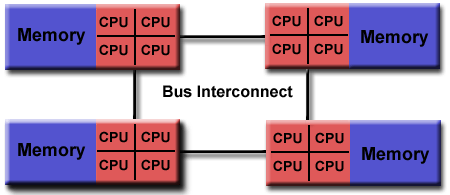
\includegraphics[width=0.92\textwidth]{./images/parallel_programming/numa}
				\caption[]{}%
			\end{subfigure}%
		\label{fig:UMA_NUMA}
		\end{figure}
		

	\end{itemize}
	SM architecture provides an easy perspective to memory,	data sharing across processors, and parallelism since no explicit communication is involved. Memory access and communication are fast due to the proximity of memory to CPUs, but it is not scalable because adding more CPUs to the pool can geometrically increases the traffic on the bus and makes cache management harder. Is up to the programmer to ensure the correct accesses to global memory in order to avoid race-conditions.
	As an example of real SM modern processor Figure \ref{fig:intelPhi} shows the Intel \textit{Knights Landing} Architecture for the intel Phi processor family which is armed with 72 cores, $8$ billions transistors at \SI{14}{\nano\metre}, AVX-512 and is able to executes 240 threads simultaneously.
		\begin{figure}
		\centering
		\label{fig:distribuiteMemory}
		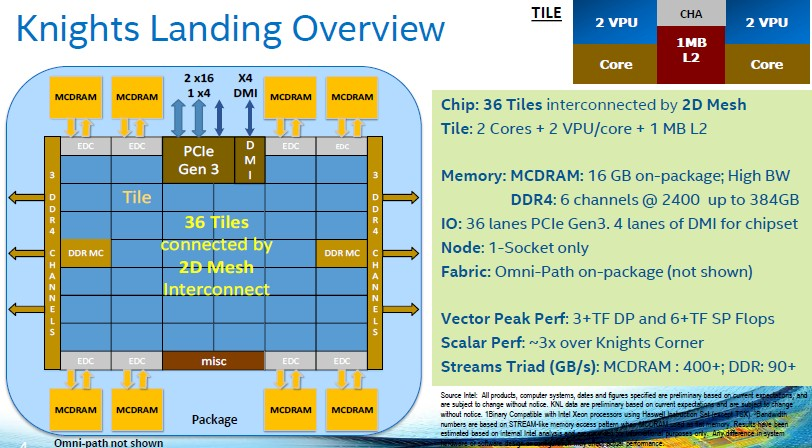
\includegraphics[width=1.0\textwidth]{./images/parallel_programming/xeonphi}
		\caption{Xeon Phi, Intel Knight Landing architecture and specifications.}
	\end{figure}
	Coupled with this architecture many software solution can be used to program
	shared memory machines. The most used are:
	\begin{itemize}
		\item Threads. Lightweight processes but with same PID (e.g. pthreads)
		\item A standard language with preprocessor directives to the compiler that is capable of converting the serial program in a parallel program without any (or very few) intervention by the programmer (e.g. \texttt{OpenMP}, see Section \ref{sec:openmp}).
		
	\end{itemize}
	

	\item [Distributed Memory] 	Different systems, and hence, different multiprocessors connected via some kind of network (see Figure \ref{fig:distribuiteMemory}), usually high speed networks such as gigabit Ethernet, InfiniBand and Myrinet, and the memory space in one processor do not map to another processor. Each of them operate independently on its memory address, so changes are not reflected on memory spaces of the others. Explicit communication is required between processors and is like synchronization	programmer's responsibility.
	This architecture  is very scalable and there is not  overhead in maintaining	cache coherency. 	
	The most used paradigm for programming distributed memory machines is the
	message passing\footnote{\texttt{MPI} is the \textit{de facto} industry standard for
	message passing. \url{http://www.mpi-forum.org/}}.
	\begin{figure}
		\centering
		\caption{Distributed memory architecture.}
		\label{fig:distribuiteMemory}
		\setlength{\fboxrule}{1pt}%
		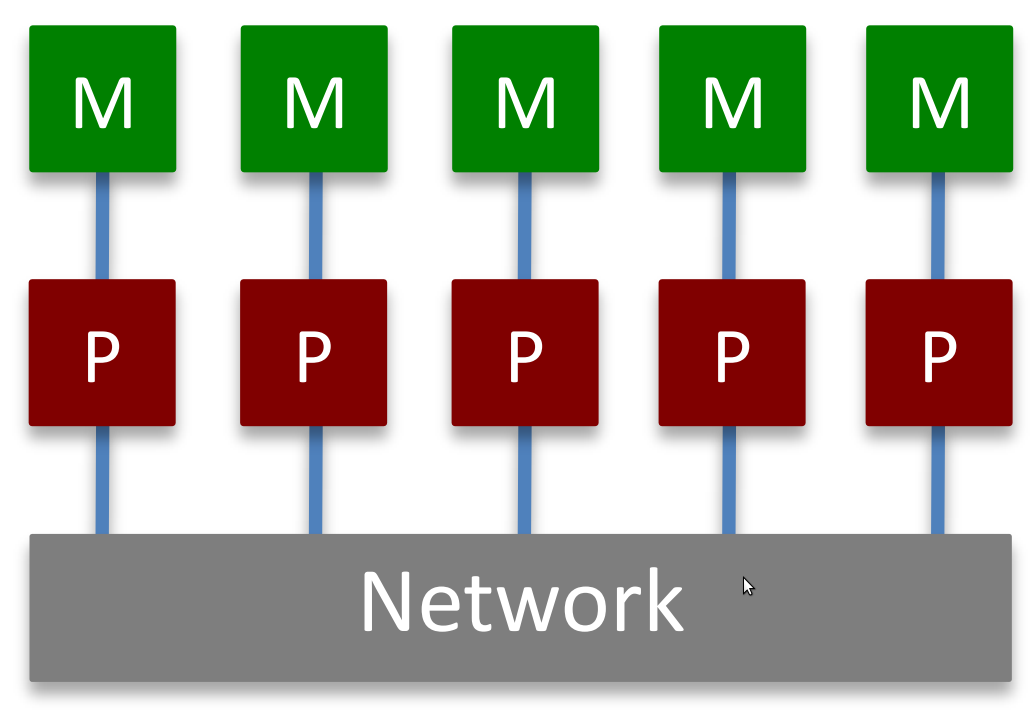
\includegraphics[scale=0.25]{./images/parallel_programming/distribuitedMemory}
	\end{figure}
	
	\item[Hybrid Systems] As the name suggest is a mix of actitectures. Only a limited number of  processors, say $N$, have	access to a common pool of shared memory. These N processor are connected to the others via network and each processor can consist of many cores.
	A common example of a  programming model for hybrid system is the combination 	of the message passing model (\texttt{MPI}) with the threads model (\texttt{OpenMP}) in which
	\begin{itemize}
		\item threads perform computationally intensive task, using local
		\textbf{on-node} memory space and
		\item communications between processes on different nodes occurs over network using \texttt{MPI} (see figure \ref{fig:hybridMemory}).
	\end{itemize} 
\begin{figure}
	\centering
	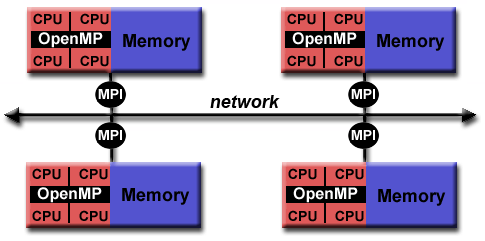
\includegraphics[width=1.0\textwidth]{./images/parallel_programming/hybrid_model}
	\caption{Hybrid memory architecture (Each processor is milti-core)}
	\label{fig:hybridMemory}
\end{figure}
	
\end{description} 
\end{description}

\section{Parallel Programming Models}
\subsection{The \texttt{OpenMP} Parallel Computing Paradigm for Shared Memory Computers}
    \texttt{OpenMP} is a portable API providing compiler directives and library
    functions for shared memory parallel programming in \texttt{C/C++} and
    Fortran \cite{Chapman:2007:UOP:1370966} implemented on top of \texttt{pthread}. It implements the
    multi-threaded \emph{fork-join} (see Figure \ref{fig:omp_fork-join}) programming model, where an initial (or master) thread forks a given number of new threads (team of threads), which share the resources of the process which they are part of and run concurrently on the available processing
    elements. Threads created during the fork phase can therefore
    rejoin to the master thread (join phase), and more fork-join
    stages can occur in a typical execution of an \texttt{OpenMP} program.
\begin{figure}
	\centering
	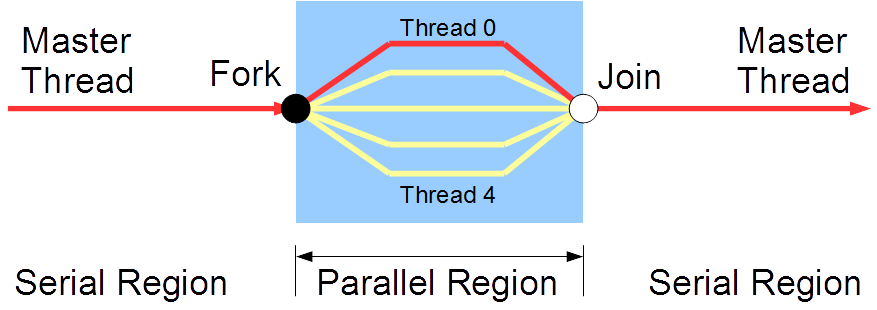
\includegraphics[scale=0.8]{./images/parallel_programming/omp_fork-join}
	\caption{\texttt{OpenMP} fork-join execution model.}
	\label{fig:omp_fork-join}
\end{figure}


    The fork-join model allows for the selective parallelization of
    the original source code (e.g. loops), by leaving portions that
    are difficult to be parallelized or that would lead to negligible
    (or even worsening) improvements, unchanged with respect to the
    serial implementation. By default, iterations are equally
    subdivided in chunks and statically assigned to threads by a
    round-robin policy. However, iterations can also be assigned to
    threads on demand, by using the dynamic scheduling clause. In this
    manner, when a thread terminates its current chunk, it requests a
    new one in a typical master-slave manner, usually resulting in
    better performance in the case chunks are not well balanced.

    Moreover, \texttt{OpenMP} provides locks to serialize the access to shared
    variables by defining critical sections. A lock must be firstly
    initialized and then can be acquired or released. When a thread
    attempts to acquire a lock that is already be set by another
    thread, its execution is suspended until the lock is released,
    giving rise to performance degradation (or even to possible deadlock
    situations). However, a lock can also be queried in order to
    evaluate its state, without blocking the thread execution. In this
    way, if the lock is already set, the querying thread can perform
    other computation, by minimizing the idle time.

    In addition to the data-type parallelization provided by the
    fork-join model, \texttt{OpenMP} aslo supports the functional-type
    parallelization, where different portions (regions) of code to be
    processed are assigned to different threads. In both cases, \texttt{OpenMP}
    parallelization of a code is straightforward, by hiding most
    low-level implementation details. Moreover, by using \texttt{OpenMP} it is
    possible to build the same source code to produce both parallel or
    sequential executable. In the latter case, the compiler simply
    ignores the \texttt{OpenMP} directives.
    
    
    \subsection{General Purpouse GPU Computing - GPGPU}
    The concept of many processor working together in concert is not new in computer graphics. Since the demand generated by entertainment started to grow, multi-core hardware emerged in order to take advantage of the high amount of parallel work available during in the processo of generating and rendering 3D images.
    In computer graphics, the process of generating a 3D images consist of
    refreshing pixels at rate of sixty or more $\si{Hz}$. Each has to be processed goes through a number of stages, and this process is commonly referred to as the \emph{graphic processing pipeline}. The peculiarity of this task is that the  computation each pixel is independent of the other's so this work is perfectly suitable for distribution over parallel processing elements. To support extremely fast processing of large graphics data sets (which mainly consists of vertices and fragments), modern GPUs employ a stream processing model with parallelism.
    The game industry boosted the development of the GPU, that offer now greater
    performance than CPUs and are improving faster too (see Figure
    \ref{CPU-VS-GPU_GFLOP} and \ref{CPU-VS-GPU_MEMORY}).
    The reason behind the discrepancy in floating-point capability between CPU and  GPU is that GPU is designed such that more transistors are devoted to data  processing rather than caching and flow control.
    
    \begin{figure}
    	\centering
    	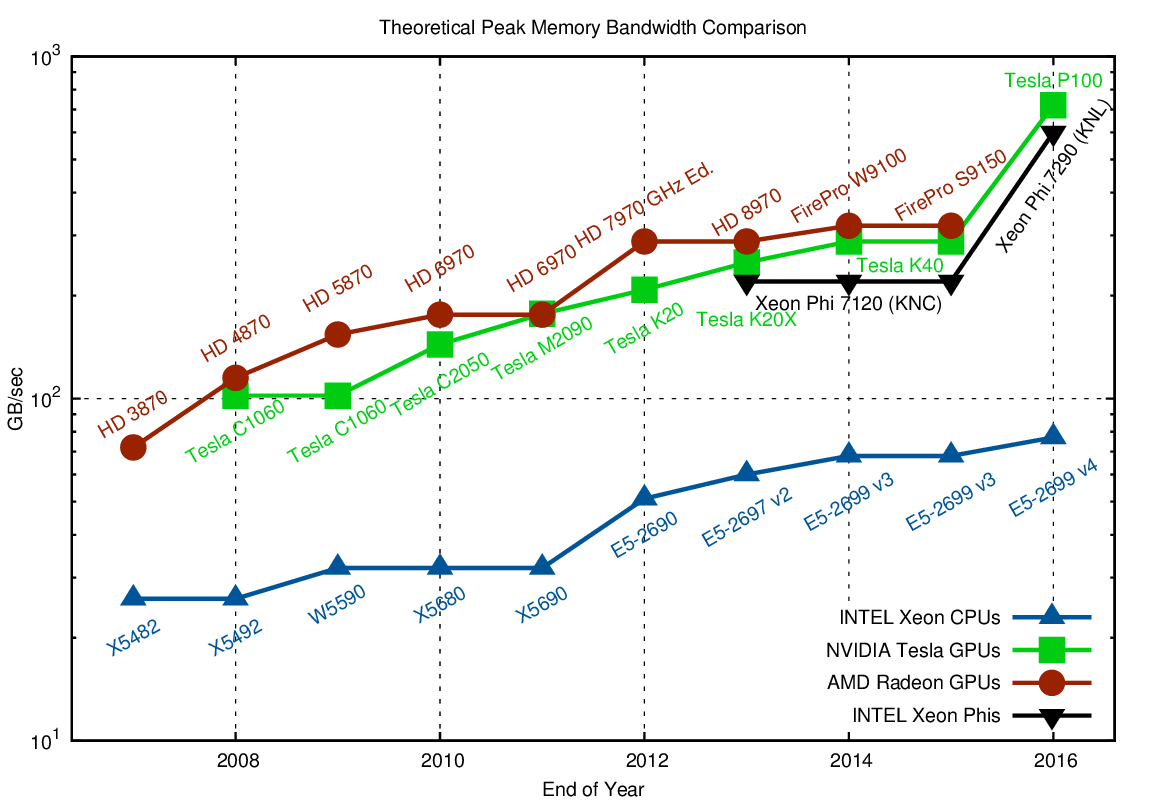
\includegraphics[width=1.0\textwidth]{./images/parallel_programming/memory-bandwidth}
    	\caption{Intel CPUs and Nvidia GPUs memory bandwidth
    		chart}\label{CPU-VS-GPU_MEMORY}
    \end{figure}
    \begin{figure}
    	\centering
    	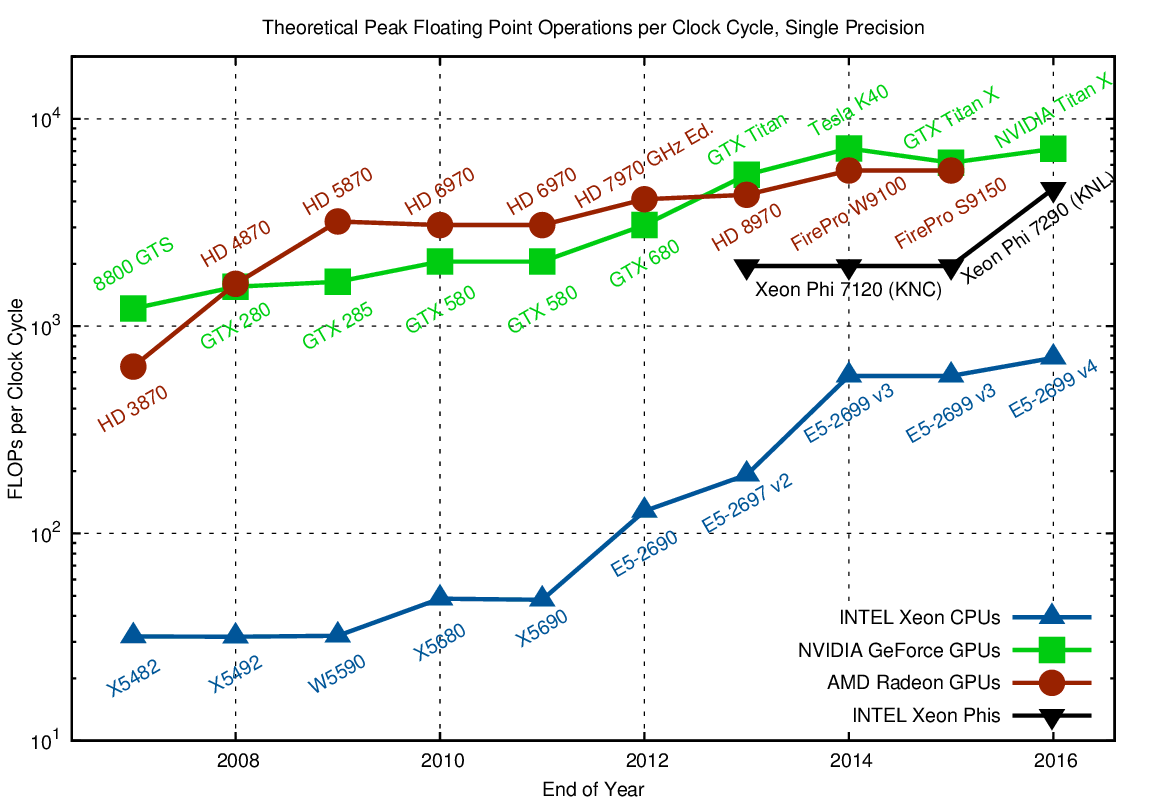
\includegraphics[width=1.0\textwidth]{./images/parallel_programming/cpu-vs-gpu}
    	\caption{Performance comparison between CPU and modern accelerators (NVIDIA, Intel and AMD) over time.}\label{CPU-VS-GPU_GFLOP}
    \end{figure}
    Nowadays, GPU are widely used for general purpouse computing. The Top 500 Supercomputers\footnote{\url{http://www.top500.org/statistics/list/}} ranking is dominated by massively parallel computer, built on top of superfast networks and millions of sequential CPUs working in concert but as the industry is developing even ore powerful, programmable and capable GPUs in term of GFlops  we see that they begin to offer advantages over traditional cluster of computers in terms of economicity and scalability.
    
    \subsection{From Graphics Graphics to General Purpose HW}\label{graphicPipeline}
    A graphics task such as rendering a 3D scene on the GPU
    involves a sequence of processing stages (i.e. shaders) that run in parallel
    and in a prefixed order, known as the graphics hardware
    pipeline\footnote{The pipeline is the most common form of 3D computer rendering, distinct from for instance, \textit{raytracing} or \textit{raycasting} for which the concept of pipeline is not even defined.}. Figure \ref{graphicPipeline} shows the important key steps that make up the graphic pipeline and for which the GPU hardware has been specialized for years. The pipeline works taking as input graphics primitives, each stage forward its results on to the next stage.
    \begin{itemize}
    	\item     The first stage of the pipeline is the \textit{vertex shader}. The
    	input to this phase is a list of vertices in object space coordinate which are then converted to world coordinates (applying the \textit{model and view matrices}).
    	\item  Shape assembly is performed where vertices are grouped together by forming graphics primitives, i.e. lines, point, polygons, triangles, tringles strips etc. If enabled, lighting calculation are also performed for each vertex.
    	\item   The following step, the \textit{geometry shader} is optionally programmable in the \texttt{openGL} pipeline and can be used to produce or delete primitives. One of the most common use of this shader is in reducing the communication between the GPU and the CPU. For instance one can only pass to the graphic pipeline a list of vertices for drawing cubes, and produce the primitives for them only when the the geometry shader is executed, reducing the amount of information exchanged between the CPU and the GPU.
    	\item   Each of the (from the now final list of) primitives is scan-converted or rasterized generating a set of fragments in screen space for the visible only part of the shapes. Each fragment stores the state information needed to update a pixel and are obtained by interpolating per vertex attributes coming from the geometry shader. For instance, each vertex of a triangle end up having its color changed based on the the color of its neighbors. 
    	\item  In the \textit{fragment  shader} is used to calculate the final color of each individual fragment. Texture coordinates of each fragment are used to fetch colors of the appropriate texels (texture pixels) from
    	one or more textures. Further Interpolation may also be
    	performed to determine the ultimate color for the fragment.
    	\item Finally, various tests (e.g., \textit{depth} and \textit{alpha}, etc.) are conducted to determine whether or how the fragment should be used to update a pixel in the frame buffer.    
    	Each shader in the pipeline performs a basic but specialised operation on the
    	vertices as it passes. 
    \end{itemize}

    In a shader based architecture the individual shader processors exhibit very limited capabilities beyond their specific purpose.
    Before the advent of CUDA in 2006 most of the techniques for non-graphics
    computation on the GPU took advantages of the programmable fragment processing stage. The steps involved in mapping a computation on the GPU are
    as follows:
    \begin{figure}
    	\centering
    	\caption{Typical graphic pipeline}\label{graphicPipeline}
    	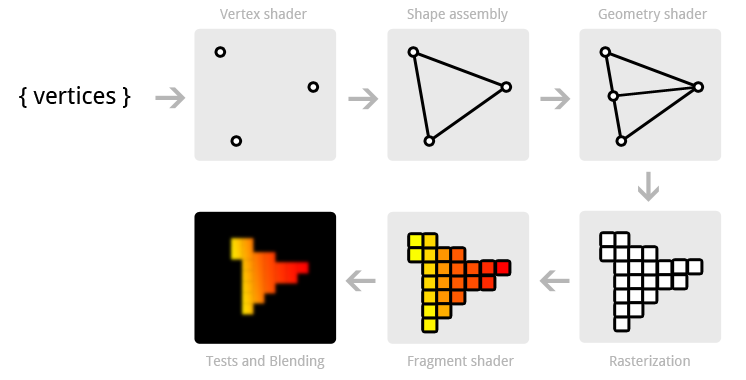
\includegraphics[width=1.0\textwidth]{./images/parallel_programming/pipeline}
    \end{figure}
    
    \begin{enumerate}
    	\item The data are laid out as texel colors in textures;
    	\item  Each computation step is implemented with a
    	user-defined fragment program. The results are encoded as pixel 
    	colors and rendered into a pixel-buffer\footnote{ A buffer in GPU memory
    		which is similar to a frame-buffer.}; 
    	\item Results that are
    	to be used in subsequent calculations are copied to textures for temporary storage and the process could start over again for another iteration.
    \end{enumerate} 
    
    The year 2006 marked a significant turning point in GPU architecture. The \texttt{G80}  was the first NVIDIA GPU to have a unified architecture whereby the different shader processors were  combined into unified stream processors. The resulting stream processors had to be more complex so as to provide all of the functionality of the shader processors they replaced. Although research had been carried out into general purpose programming
    for GPUs previously, this architectural change opened the door to a far wider range of  applications and practitioners.    
    GPUs are nowadays, well-suited data-parallel problems because they are very good at execution the same code on many data elements at the same time  in a \textit{Single Instruction, Multiple Threads} (SIMT) fashion or using a more general definition as \textit{Parallel Random-Access Machine in which each thread Can Read or Write a memory location} (\texttt{CRCW PRAM}).
    
    
    \section{The \texttt{OpenCL} Parallel Computing Paradigm on Heterogeneous Devices}
    Released on December 2008 by the Kronos Group, \texttt{OpenCL} is an open standard for programming heterogeneous computers built from CPUs, GPUs and other processors. It allows to define the computation using the \textit{platform} abstraction. A platform is composed by an host device and one or more compute devices. A C-like language is the used to program and orchestrate the various parts of the platform (see Figure \ref{fig:openCL}).
    One of the advantages of \texttt{OpenCL} is that it is not restricted to the use of
    GPUs but it take each computing resource in the system as computational peer unit, easing the process of interfacing with them. Another big advantage is that it is an open, free cross-compatible across vendors since is supported by all major hardware producers.
    
    A typical \texttt{OpenCL} application is subdivided in two parts, one
    running on the CPU (host application) and one or more running on a
    compliant device (device application), where the actual parallel
    computation generally takes place. The host application defines
    the tasks to be executed in parallel. Each parallel task is
    implemented as an \texttt{OpenCL} \emph{kernel}, which is a special C
    function, which is specifically (runtime) compiled  and deployed to a compliant device (or even to different different devices) for execution. The execution model is similar to the one of CUDA (with different terminology), where each kernel is executed by threads, the smallest execution entity, also called work-items, which are grouped into work-groups. A work-item is executed by one or more processing elements as part of a work-group executing on a compute unit. A work-item is distinguished from other executions within the collection by its global ID and local ID.
    A Work-group is a collection of related work-items that execute on a single compute unit. The work-items in the group execute the same kernel and share local memory and work-group barriers.
    Work-groups can 
    \begin{itemize}
		\item Share data between the work-group's work-items using local memory
		\item Synchronize between work-items using barriers and memory fences mechanism
		\item Use special built-in functions such as \texttt{work\_group\_copy}
    \end{itemize}

    \begin{figure}
	\centering
	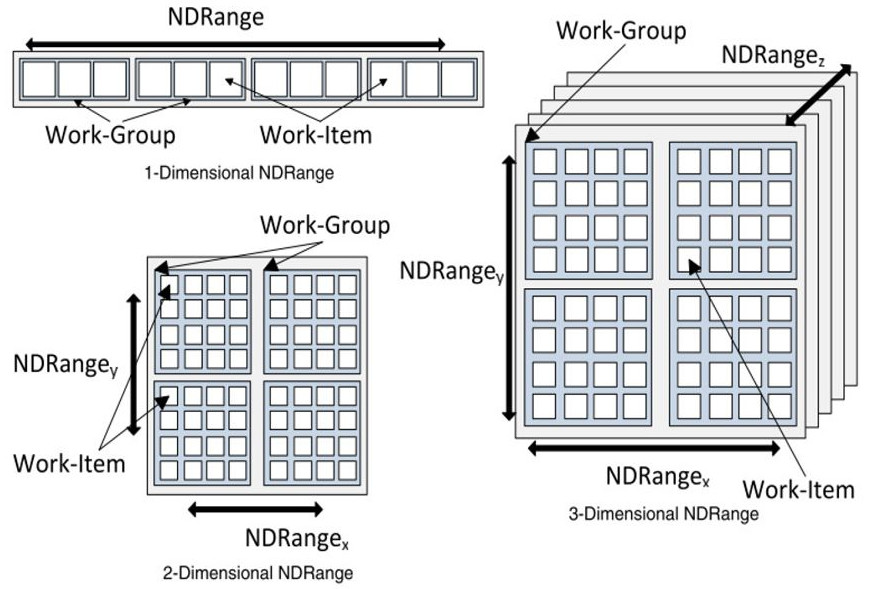
\includegraphics[width=1.0\textwidth]{./images/parallel_programming/opencl_execmodel}
	\caption{\texttt{OpenCL} 1D,2D,3D work-items and work-groups partitioning. }\label{fig:opencl_execmodel}
\end{figure}


    When launching the kernel for execution, the host code defines the grid dimensions, or the global work size. The host code can also define the partitioning to work-groups, or leave it to the implementation. During the execution, the implementation runs a single work item for each point on the grid. It also groups the execution on compute units according to the work-group size. The order of execution of work items within a work-group, as well as the order of work-groups, is implementation-specific.
    Data to be processed has to be explicitly partitioned and assigned to compute units because each work-item runs the same kernel on different portions of data in a \textit{SIMD/SIMT} fashion. For example, in case of an array of $n$ elements and $n$ work-items, data can be partitioned by associating each work item to the array element with index corresponding to the work-item ID. Moreover, a local ID is defined for each work-item    within a workgroup. Figure \ref{fig:opencl_execmodel} depicts how items and groups can be arranged when partitioned in 1D, 2D and 3D.
    Figure \ref{fig:opencl_execmodel2d} shows a 2D decomposition with details on global ID computation from local group and thread indices.
    
        \begin{figure}
    	\centering
    	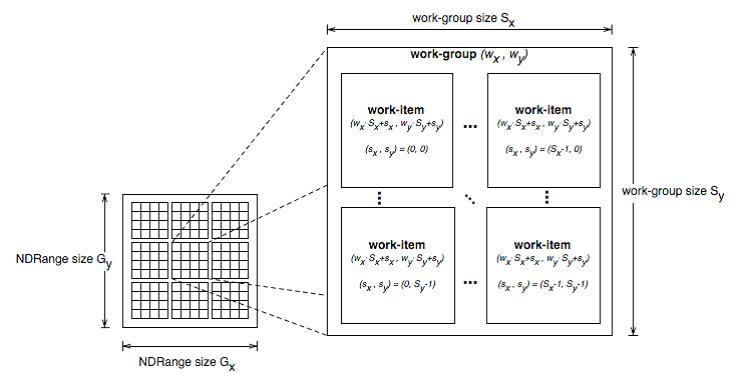
\includegraphics[width=1.0\textwidth]{./images/parallel_programming/opencl_execmodel2d}
    	\caption{\texttt{OpenCL} 2D work-items and work-groups detailed partitioning. Computation of global index form local item and group index is also shown. }\label{fig:opencl_execmodel2d}
    \end{figure}
    When the kernel execution terminates,
    work-items globally synchronize, and the control returns to the
    host application. Similarly to the OpenMP fork-joins stages,
    different kernel executions and synchronization stages can take
    place in a typical \texttt{OpenCL} application.
    
    Data can be shared by all the running threads by means of the
    device global memory, which is generally the larger among the
    different memory levels available on the device (e.g. on GPUs)
    though being the slower one. A read-only memory, equivalent to the
    global one in terms of latency and dimension, called constant
    memory, is also available. Some devices have an appropriate
    portion of this memory, while in other cases the constant memory
    space coincides with that of the global memory. Threads within a
    workgroup are executed by a specific compute unit and therefore
    can share data on the local memory and also synchronize each
    other. Local memory is generally smaller with respect to the
    global one, but allows for faster access (about $100\times$ faster
    on modern GPUs). Eventually, each work-item has its own private
    memory, which is at the same time the fastest and the smaller
    one. The memory space in which a given data must be stored must be
    initially defined by the host. However, data can move among
    different memory levels during kernel execution.
    
    Data exchange and kernels execution are managed host-side thanks
    to an \texttt{OpenCL} context. In particular, the host application links
    kernels into one or more containers, called \emph{programs}. The
    program therefore connects kernels with the data to be processed
    and dispatches them to a special \texttt{OpenCL} structure called
    \emph{command queue}. This is necessary because only enqueued
    kernels are actually executed. The context contains all the
    devices, command queues and kernels, each device has its own
    command queue and each command queue contains the kernels to be
    executed on the corresponding device. Moreover, an \texttt{OpenCL}
    application can configure different devices to perform different
    tasks, and each task can operate on different data. \texttt{OpenCL}
    provides thus a full task-parallelism. Command queues are also
    used for host-device and device-device data transfer operations,
    synchronization between different kernels, and profiling
    operations.
    
    
	Kernels are usually listed in separate
    files the \texttt{OpenCL} runtime use to create kernel object that
    can be first decorated with the parameters on which it is going to
    be executed and then effectively enqueued for execution onto device.
    
    The following is a brief description of the typical flow of an \texttt{OpenCL} application (See Figure \ref{fig:opencl_program_flow}).
    \begin{figure}
    	\centering
    	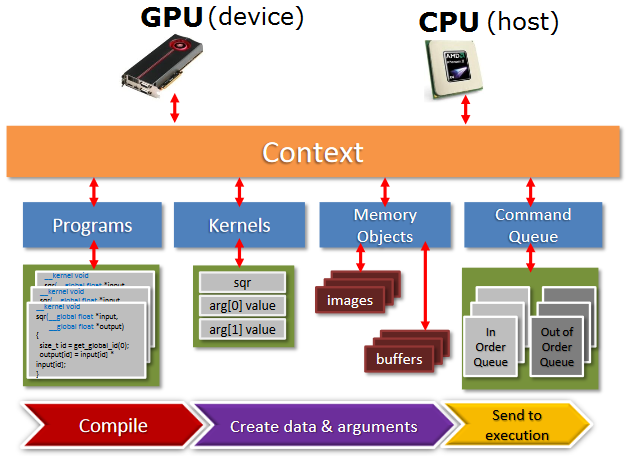
\includegraphics[width=1.0\textwidth]{./images/parallel_programming/opencl_program_flow}
    	\caption{\texttt{OpenCL} program flow and interaction between memory, device and host.}\label{fig:opencl_execmodel}
    \end{figure}

    \begin{enumerate}
    	\item Contexts creation: The first step in every \texttt{OpenCL} application is to create a context and associate to it a number of devices, an available \texttt{OpenCL} platform (there might be present more than one implementation), and then each operation (memory management, kernel compiling and running) is performed within \emph{this} context. In the example \ref{code:openCLContext} a context associated with the CPU device and the first finded platform is created.\\

    	\item Memory buffers creation: \texttt{OpenCL} buffer Object are created. Those
    	buffer are used to hold data to be computed onto devices.\\
    	
    	\item Load and build program: we need to load and build the compute program
    	(the program we intend to run on devices). The purpose of this phase is to
    	create an object \textbf{\textit{cl::Program}} that is associable with a
    	context and then proceed building for a particular subset of
    	context's devices. We first query the runtime for the available devices and
    	then load directly source code as string in a
    	\textbf{\textit{cl::Program:Source}} \texttt{OpenCL} object (see listing1
    	\ref{code:loadBuildProgramCL}).\\
    	
    	\item In order a kernel to be executed a \emph{kernel object} must be created.
    	For a given \emph{Program} there would exists more than one entry point
    	(identified by the keyword \emph{\_\_kernel} \footnote{Obviously in the same
    		source code one can define more than on kernel.}). We choose one of them for
    	execution specifying in the kernel object constructor\\
    	
    	\item We effectively execute the kernel putting it into a 
    	\emph{cl::CommandQueue}. Given a cl::CommandQueue queue, kernels can be queued
    	using \textit{queue.enqueu\-NDRangeKernel} that queues a kernel on
    	the associated device.
    	Launching a kernel need some parameters (similar to launch configuration in
    	CUDA, see section \ref{kernels}) to specify the work distribution among
    	work-groups and their dimensionality and size of each dimension (see listing
    	\ref{code:openCLQueuCommand}). We can test the status of the execution by
    	querying the associated \emph{event}.\\
    \end{enumerate}
    
    
    \lstset{language=[OpenCL]C,
		caption={\texttt{OpenCL} Queue command,
		kernel execution}, 
    	label={code:openCLQueuCommand}, 
    		basicstyle=\ttfamily,
    	keywordstyle=\color{blue}\ttfamily,
    	stringstyle=\color{red}\ttfamily,
    	commentstyle=\color{green}\ttfamily,
    	backgroundcolor=\color{light-gray}, 
    	numbers=left, 
    	numberstyle=\tiny
    }
    \begin{lstlisting}
    cl_int err;
    cl::vector< cl::Platform > platformList;
    cl::Platform::get(&platformList
    checkErr(platformList.size()!=0 ?  \\
    CL_SUCCESS:-1,"cl::Platform::get");
    cl_context_properties cprops[3] =
    {CL_CONTEXT_PLATFORM, (cl_context_properties)(platformList[0])(), 0};
    cl::Context context(CL_DEVICE_TYPE_CPU,cprops,NULL,NULL,&err);
    checkErr(err, "Conext::Context()"); 
    \end{lstlisting}
    
     \lstset{language=[OpenCL]C,
     	caption={\texttt{OpenCL} context creation}, 
    	label={code:openCLContext}, 
    	    	keywordstyle=\color{blue}\ttfamily,
    	stringstyle=\color{red}\ttfamily,
    	commentstyle=\color{green}\ttfamily, 
    	backgroundcolor=\color{light-gray}, 
    	numbers=left, 
    	numberstyle=\tiny
    }
    \begin{lstlisting}
    cl::Buffer outCL(context,CL_MEM_WRITE_ONLY |
    CL_MEM_USE_HOST_PTR,hw.length()+1,outH,&err);
    checkErr(err, "Buffer::Buffer()");
    \end{lstlisting}
    
     \lstset{language=[OpenCL]C,
       	caption={\texttt{OpenCL} program load and build}, 
    	label={ code:loadBuildProgramCL}, 
    	    	keywordstyle=\color{blue}\ttfamily,
    	stringstyle=\color{red}\ttfamily,
    	commentstyle=\color{green}\ttfamily,
    	backgroundcolor=\color{light-gray}, 
    	numbers=left, 
    	numberstyle=\tiny
    }
    \begin{lstlisting}
    std::ifstream file("pathToSourceCode.cl");
    checkErr(file.is_open() ? CL_SUCCESS:-1, "pathToSourceCode.cl");std::string
    prog( std::istreambuf_iterator<char>(file),
    (std::istreambuf_iterator<char>()));
    cl::Program::Sources source(1,std::make_pair(prog.c_str(), prog.length()+1));
    cl::Program program(context, source);
    err = program.build(devices,"");
    checkErr(err, "Program::build()");
    \end{lstlisting}
    
     \lstset{language=[OpenCL]C,
	caption={\texttt{OpenCL} program load and build}, 
	label={ code:loadBuildProgramCL}, 
	keywordstyle=\color{blue}\ttfamily,
	stringstyle=\color{red}\ttfamily,
	commentstyle=\color{green}\ttfamily,
	backgroundcolor=\color{light-gray}, 
	numbers=left, 
	numberstyle=\tiny
}   
    \begin{lstlisting}
    cl::CommandQueue queue(context, devices[0], 0, &err);
    checkErr(err, "CommandQueue::CommandQueue()");cl::Event event;
    err = queue.enqueueNDRangeKernel(kernel,cl::NullRange,
    cl::NDRange(hw.length()+1),	cl::NDRange(1, 1),NULL,&event);
    checkErr(err, "ComamndQueue::enqueueNDRangeKernel()");
    \end{lstlisting}
%%%%%%%%%%%%%%%%%%%%%%%%%%%%%%%%%%%%%%%%%%%%%%%%%%%%%%% 
\subsection{The Message Passing Interface}


    